\documentclass[11pt]{article}
\usepackage{lscape}
\usepackage[table]{xcolor}% http://ctan.org/pkg/xcolor
\setlength{\parindent}{0pt}
\usepackage [colon]{natbib}
\usepackage {comment}
\renewcommand{\familydefault}{\sfdefault}
\usepackage[a4paper, margin=2.40cm]{geometry}
\usepackage{doi}
\usepackage{multirow}
\usepackage[T1, OT1]{fontenc}
\DeclareTextSymbolDefault{\dh}{T1}
\renewcommand{\rmdefault}{phv} % Arial
\renewcommand{\sfdefault}{phv} % Arial
\usepackage[modulo]{lineno}
\usepackage{wrapfig}
% \linenumbers
\usepackage{hyperref}
\usepackage{array}
\newcolumntype{L}[1]{>{\raggedright\let\newline\\\arraybackslash\hspace{0pt}}m{#1}}
\newcolumntype{C}[1]{>{\centering\let\newline\\\arraybackslash\hspace{0pt}}m{#1}}
\newcolumntype{R}[1]{>{\raggedleft\let\newline\\\arraybackslash\hspace{0pt}}m{#1}}
\usepackage{amsmath}
\usepackage{float}
% \errorcontextlines=3
\usepackage[explicit]{titlesec}
\usepackage{graphicx}
\usepackage{caption}
\usepackage{authblk}
\usepackage{setspace}
\usepackage[export]{adjustbox}
\renewcommand{\bibfont}{\footnotesize}
\usepackage{bibentry}
\usepackage{tikz}
\usepackage[inline,shortlabels]{enumitem}
\usepackage[all]{nowidow}



\newcommand{\TODO}[1]{\textbf{TODO #1}}
\newcommand{\ian}[1]{{\textbf{\color{blue}Ian says:} \color{blue} #1} }
\newcommand{\leif}[1]{{\textbf{\color{red}Leif says:} \color{red} #1} }
\newcommand{\frederic}[1]{{\textbf{\color{red}Frederic says:} \color{red} #1} }
\newcommand{\aref}[1]{\textbf{Reference #1}}
\newcommand{\alpine}{\textit{ALPINE}\,}
\newcommand{\icesheet}{\textit{ICESHEET}\,}
\title{}
\author{}

\begin{document}
Dear Editor,

\vspace{.2cm}

We thank Reviewer 1 for their detailed and constructive comments. Their work, we believe, has provided feedback that has greatly improved the manuscript.

\vspace{.2cm}

The reviewer's comments are in bold, our response is in italics and quotations from the new text are in normal font.

\vspace{.3cm}

Best regards,

\vspace{.75cm}

Ian Delaney on behalf of all authors

\vspace{2cm}

\textbf{General Comments}

\begin{itemize}

\item \textbf{In my view the paper is interesting and relevant, and hence worthy of publication. I have a couple
    of general observations, followed by a list of minor suggestions.
    My general observation relates to the structure of the main findings reported by the manuscript.
    In reading the Results and Discussion I was sometimes lost as to what I was learning that was new.
    I think this was mainly because the structure lacked a clear and logical progression from one
    general finding through progressively more specific findings. This may well stem an initial
    imperfect expression of the objectives.}

  \textit{We thank the Reviewer for their positive assessment of our work and acknowledge the structural and organizational issues they have highlighted.}
  
\item  \textbf{Here, most of what is novel seems to fall under Objective
    2 and not under Objective 1. Indeed, isn’t Objective 1 (‘to establish whether sub-seasonal water
    discharge can co-vary with sediment transport capacity in subglacial systems’) already established
    beyond reasonable doubt? To me, and I believe the introduction to this manuscript, it clearly
    ‘can’… (note the objective refers to ‘can it’, and not to ‘does it’ [to which the answer is also almost
    certainly ‘yes’ but perhaps with a little more room for maneuver]). I would recast the objectives
    to reflect better the new material presented in this manuscript (closer to objective 2 in fact, which
    I feel could readily be sub-divided). Having considered this, I feel the progression of the Results
    could be far more accessible to the reader and allow the manuscript to focus on a few really key
    points (which I think are currently slightly lost in the density of the presentation).
    Interpretation is presented within each Results section (e.g., see ‘due to… on L174). This
    continues throughout Results, and I would separate all of the explanation and hence
    interpretation out form the results.}

  \textit{We greatly appreciate this comment. After careful consideration, we have chosen to rephrase Objective One as:} ``to establish the hydrological conditions under which sediment transport capacity co-varies with water discharge in subglacial systems.'' 

\textit{In our view, this objective directs attention to the differences between the ALPINE and ICESHEET scenarios. It is also practical for evaluating the effects of water discharge smoothing, as discussed in the next point.}

\textit{We acknowledge the importance of removing interpretation from the results section and have made the necessary revisions. Additionally, we will moved Section 4.3, which contains the algebraic formulations, to the discussion section, as we believe that the pipe flow and steady-state R-channel scenarios serve as useful end members for interpreting the results.
}


  
\item \textbf{There are some very important points in Results, which I would attach some key data to
    and make more explicit here and in the Conclusion and Abstract. I’m thinking for example of
    associating the (increased) hysteresis as a function of discharge with a headline \% change in
    sediment transport capacity. E.g., “thus, a more variable, but typical, Alpine Q record can
    transport up to *\% greater sediment per cumec than a less variable ice sheet-type Q” and/or “the
    greater variability in Q from Alpine than from ice sheet style Q can account by an offset of peak
    sediment discharge from peak meltwater discharge by up to * \% of the cycle involved”. At present,
    I feel the manuscript lacks this incisive illustration to bring the scale of the results home to the
    reader.}

  \textit{This is an excellent comment, and we have worked to provide a clearer explanation of hysteresis.}

\textit{One challenge with the approach recommended by the reviewer is that sediment transport capacity scales highly non-linearly with water discharge, particularly in subglacial systems, as demonstrated in Section 4.3. Consequently, findings across different hydrographs would not be directly comparable, even if they were scaled using a discharge quantity.}

\textit{Instead, we have added several paragraphs to Section 4.1 discussing the role of water discharge variability in hysteresis.}

  \textit{Here the aim is to evaluate the effects of smoothing hydrographs, yielding insights in to the hydrological conditions where discharge and sediment transport capacity can co-vary.
    Note that the smoothed hydrographs used for the analysis here are presented in the supplement. 
    A version of the new paragraphs is as follows.}


\begin{figure}[H]
  \centering
  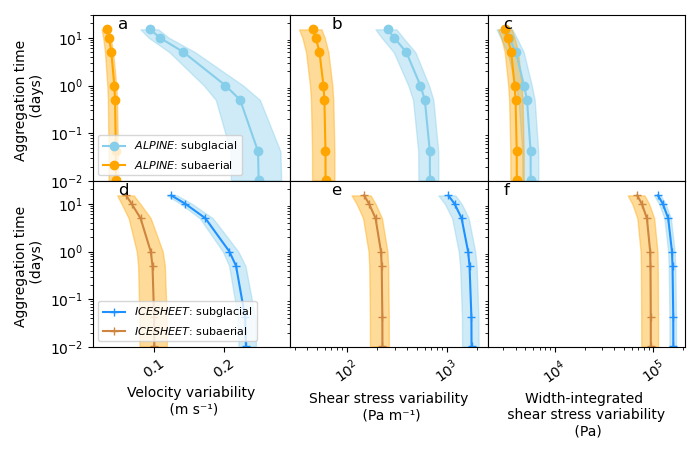
\includegraphics[width=0.8\linewidth]{../Fig4.png}
  \caption{Spearman rank correlation between water discharge over a smoothed period and sediment transport characteristics (a) water velocity, (b) shear stress, (c) width-integrated shear stress. Higher correlation scores mean reduced hysteresis and approach subaerial behavior.
  }
  \label{fig:corri}
\end{figure}

  
Water discharge and sediment transport characteristics correlate better in \icesheet{} with lower diurnal variations in water discharge compared to the \alpine{}.
To evaluate the impact of water discharge variability, we smoothed the two hydrographs across different periods and evaluated the Spearman rank correlation between sediment transport characteristics and water discharge.
We assume that a higher rank correlation indicates a reduced amount of hysteresis and behavior more similar subaerial channels (Figure~3).

Smoothing water discharge over periods longer than one day causes a substantial increase in rank correlation (Figure~5).
This increase occurs as diurnal variations are removed (Figures S1-S14).
Correlations in sediment transport characteristics in \icesheet{} remain higher than \alpine, which has more water discharge variations even when smoothed compared to \icesheet{} (Figure~S1-S14).  

  
\item \textbf{Less importantly, but something I’d like to check, is that the fundamental conclusions are
    applicable more generally. Since they derive from modelling based on two ‘type’ datasets, there
    may be a possibility that not all key findings hold for certain other variations of subglacial
    discharge pattern. I have every reason to believe they do, but I feel the manuscript should report
    that this has been done more widely and the key results/patterns still hold. I don’t think there’s
    any need to include any such results into a revised manuscript – but I would just make the
    statement that while, for simplicity of illustration, two typical but contrasting datasets are
    explored here, the model has been run with other data sets and the key do hold more generally.}

  \textit{We thank the reviewer for this comment as it, in part, encouraged us to add the additional section above with the water discharge smoothing.
    The other hydrological scenario we are aware of not explicitly considered here is Antarctica, where little surface melt occurs.
    Thus, we expect variations in water discharge to be minimal.
    The following sentence has been added to the conclusion:}
    ``Water discharge and sediment transport capacity covariance could be possible when water discharge varies at a slower rate than subglacial channel size, such as in Antarctica with minimal surface melt input.''
    
\item   \textbf{
    Incidentally, I would also include an explicit disclaimer early on that the analysis only relates to
    pressurized subglacial flow and not to open-channel flow prominent approaching the terminus of
    many valley glaciers etc.}

   \textit{ We will add the following sentence to the model implementation section:}
``We also note that the subglacial results apply to pressurized subglacial channels, not depressurized one that can occur below glacier termini \citep{perolo2018}''
\end{itemize}

\textbf{Specific Comments}

\begin{itemize}
\item \textbf{Title:}The title states the obvious from prior research and I would recast it to
  reflect more accurately the new and original contribution of this
  manuscript. Also, if the authors elect to not change the title I would change
  the existing wording to ‘transport capacities respond differently’.
  Grammatically, this is not clear given the two capacities noted earlier in the
  title, but stylistically I think ‘capacities respond’ reads better than does
  ‘capacity respond’. (I would change the whole thing anyway… Why not start
  by considering ‘Sediment transport capacity response to variations in water
  discharge in pressurized subglacial channels’)

  \textit{Excellent suggestion, the title follows the reviewer's suggestion:} Sediment transport capacity response to variations in water discharge in pressurized subglacial channels
  
\item \textbf{3:} ‘full’ subglacial channels?

  \textit{Done.}
  
\item \textbf{5:} There is no need to mention ‘over days’ here (indeed, it is misleading
  anyway without quantification of how much change as a function of time).
  I would just leave it as changes slowly (or slowly relatively to variations in
  water Q).

  \textit{Done.}

\item \textbf{7:} ‘Sheet’ is missing (the authors really should have picked up on this obvious
  typo)

  \textit{Done.}

  
\item \textbf{8:} This hysteresis causes (no need to qualify the type of hysteresis since the
  use of ‘this’ serves the purpose)

  \textit{Done.}

  
\item \textbf{64:} I think there is earlier use of transport-limited (in which case the definition
  should be presented there, and not here)

  \textit{We thank the reviewer for the careful read. The definition was presented in Line 28, and thus we will remove the definition here.}


\item \textbf{75-76 and 80-81} I’d remove summary of the results of this study from the Introduction. They
  are not yet established.

  \textit{These lines will be removed.}

\item \textbf{70-71} In phrasing objective 1 (in more than one place in the manuscript),
  shouldn’t the dependent variable come first? Thus, I would write it as ‘to
  establish whether sediment transport capacity can co-vary with water
  discharge in subglacial systems’.

  \textit{Given the discussion above, the text will read:} ``to establish the hydrological conditions where  sediment transport capacity co-varies with water discharge in subglacial systems''
  
\item \textbf{79} Given the apparent relevance of the Alley et al. study, I feel it’s key findings
  should be presented in detail here to provide more direction to the specific
  objectives of this study.

  \textit{We believe that this is discussed in Lines 51--54 in the introduction.}


  
\item \textbf{159} The parameter values are not purely random (but random within certain
  sensible ranges, no?).

  \textit{The text will now  read:} ``with random parameter values in a range''

\item \textbf{171-} I get a little muddled right at the start here – not helped by the sub-heading,
  which I would recast as “Influence of subglacial channel size on the timing
  and variability of…”. The section (and others following) also combines
  results with explanation (i.e., interpretation) which I feel also adds
  unnecessarily to the difficulty in following the progression. I would separate
  results from interpretation.

  \textit{This section will be retitled:} ``Timing of subaerial and subglacial sediment transport capacity variations.''
  \textit{This discusses the role of water discharge on hysteresis in water velocity or sediment transport capacity. Thus dealing with Objective One of the manuscript. We have also noted the comment about results and interpretation. These have been removed from the manuscript}
  

\item \textbf{172} This narrative jumps straight in with the ambition to ‘quantify the sources
  of increased variability…’ but the nature of that increased variability has not
  yet be established or illustrated. This really needs building up more
  progressively – bringing the reader through with the first-order model
  results. Then go on to explore more and more detailed influences and
  relationships. Most of this is, in fact, in Figure 2 – but the reader is not
  guided through the fundamental relationships here.

 \textit{Excellent comment. The first sentence of the section will read:} ``The first numerical experiment aims to quantify the timing and covariance of the subglacial model outputs with respect to water discharge in response to different seasonal evolutions and peaks''

\item \textbf{173} Change rather than evolution? (elsewhere too)

  \textit{We appreciate the comment. We believe that given the nature of subglacial channels, as described in Equation 3, evolution is a more accurate description. To us, ``change'' could include a modification for any number of reasons. However,
    ``evolution'' connotates the dependence on antecedent conditions which we believe to be more accurate in this case. }
  
\item \textbf{Fig 2 caption} Is it really an arbitrary y axis scale? If it is truly arbitrary, does it even need
  a scale range?

  \textit{We believe that a description of the insets' axis is needed as these lines have the same axis in the main plots. However, their very different values mean that it makes sense to adjust values to examine their changes during the extreme melt event. The text will be modified slightly to read:} ``different y-axis ranges for subaerial and subglacial values.''


  
\item \textbf{179-183} Is this not already established? If so, it should be presented clearly in the
  Introduction and developed as necessary here. It is also interpretation.

  \textit{ To the best of our knowledge this is the first time that this finding is being presented.
    We would welcome any citations or references that suggest otherwise. We believe that the content in this paragraph describes the response to water discharge in Figure 2. We agree that the reference to the ``Methods'' section, gave the impression of the interpretation. The paragraph will be adjusted slightly to read:}


    Peaks in subaerial model outputs occur coincident with peaks in water discharge (Figure~2).
    In the subglacial channel, peaks in model outputs generally occur when water discharge increases, but before the maximum water discharge.
    As the water discharge stabilizes at its peak, channel growth continues (Figure~2 a, e), causing water velocity and other model outputs to decrease from their peak values (Figure~2 b-d, f-h).
    Subglacial sediment transport capacity is greatest on the hydrograph's rising limb, relative to the falling limb, creating a hysteresis effect.''
  
  
\item \textbf{Fig 3 (and Fig 4)} Shouldn’t the dependent variable be plotted on y and the independent
  variable on x? I for one at least think this way around and therefore find
  these plots a little confusing.
  Is there a need for the axis labels to be at an angle rather than parallel to
  the axis? If not, I would reorientate them parallel in all cases.

  \textit{The axes will be changed in both figures}
  
\item \textbf{193-4} This is interpretation.

  \textit{This sentence will be removed.}
  
\item \textbf{195} The reference to ‘increased variability’ needs to make it clear what property
  is being referred to. Like the previous sub-heading, this sub-heading is a
  statement of findings before those results have been presented. I would
  avoid this and present it as the less assuming: ‘Influence of…’


  \textit{The section head will be modified to read:} Variability in sediment transport capacity across a range of channel shapes, slopes, and friction values

\item \textbf{205-6} Interpretation in Results

  \textit{Removed.}
  
\item \textbf{210-11} Interpretation in Results

  \textit{ Sentence will be changed to:}'' Smaller values of channel factor $\beta$, creating low and broad channels where the channel width grows more quickly in response to water discharge increases as compared to a semi-circular channel with $\beta = \pi$ (Equation~4).''
  
\item \textbf{220 Typo (subglacial)}


  \textit{Fixed.}
  
\item \textbf{Section 4.3} A lot of this reads more like methods and background modelling operation
  and/or equation terms than Results of the modelling. If it is all results then
  the key findings are difficult to pull out from the density of the presentation
  – perhaps some of it could be omitted or moved to supplementary?

  \textit{We have considered the comments here, and with the editor's support, think it fits best in the manuscript.
  However, we have moved it to the discussion to set up the end member cases of pipe flow and steady-state R-channels.
    In a previous version of the manuscript, it was included in the supplementary material. However, after those reviews, we believe that some misunderstandings emerged. We believe that Tables 2 and 3 in the section are valuable results in evaluating the sensitivity of sediment transport capacity to water discharge under different assumptions.
  }

  \textit{We will modify the introductory text to read}: ``The numerical experiments above consider the size evolution of subglacial channels and demonstrate that for these hydrographs subglacial sediment transport variability is greater than its subaerial counterpart (Section~4.3). 
Additionally, results demonstrate the impact of water discharge variability on sediment transport capacity.
Here, we compare the sediment transport behavior of different channel types as they respond to water discharge, channel shape, and hydraulic gradient.''


\item \textbf{Fig 5} I find the figure too small. If larger the font would be easier to read and the
  y axes could have the property written out rather than represented by
  symbols. I’m sure there is no need for it to be this small.

  \textit{We will increase the size of the axis labels.}

\item \textbf{232} Typo? (‘typesc’)
  \textit{Removed.}
  
\item \textbf{235} The text: ‘…as used as proxy for…’) doesn’t make sense (or at least could be
  worded more clearly).

\textit{Text will read: ''additionally width-integrated shear stress is assessed, instead of sediment transport, as above.''}
  
\item \textbf{284} (maybe
  elsewhere too)
  The wording should be “greater …. than” and not ‘greater… compared
  with…).

  \textit{Done.}

\item \textbf{297} “…itself dependent of…” doesn’t make sense to me

  \textit{Text now reads: ''which is dependent''}

\item \textbf{298} I don’t believe there is sufficient evidence to make the claim: ‘While
  transport limited states likely do not occur at many glaciers’. In my own
  experience most glacier do have at least parts of the bed that are sediment-
  rich and hence have the capacity to be transport limited.

  \textit{We agree with the reviewer about the lack of data. This sentence will be removed. }


  
\item \textbf{302-4} I would try to pull some key quantification out here and present it as a
  headline figure to illustrate the magnitude of the effect.

\item \textbf{319} I’m not sure ‘sporadic’ is the right word here. Please check you mean this.

  \textit{We will replace ``sporadic'' with ``variable''.}
  

  
\item \textbf{321-22} I see the point being made here but it’s not black or white. Surely there is
  some control exerted by discharge; it’s just that it is complicated by the
  additional forces in the subglacial scenario. The way this is presented here
  may be technically ok but the reader could be forgiven for coming away
  with the feeling that there is no solid relationship between Q and sediment
  transport capacity is these cases – which would not be accurate. I feel it
  would be particularly helpful if the effect could be quantified in some
  generalized or headline way in terms of the likely (or maximum if you
  prefer) effect on a typical alpine and/or ice sheet hydrograph. That figure
  could then also go into the Conclusions and Abstract.

  \textit{The sentence will read:} ``This hysteresis can limit water discharge as an indicator of sediment discharge capacity in these systems, especially when water discharge is highly variable and out of equilibrium with subglacial channel size.''

\item \textbf{394} Surely the relationship can be characterized a little more usefully than
  simply to state that it is ‘incoherent’. This also relates to my point above
  relating to lines 321-22. Can this be characterized accurately or
  systematically so the reader has a little more to learn in terms of the nature
  and magnitude of the effects?

\textit{This paragraph will read:} ``The manuscript's first objective is to establish the conditions where water discharge covaries with subglacial sediment transport capacity.
In subglacial channels, the timing of peak water velocity and sediment transport capacity occurs before peak water discharge during a discharge event, due to evolving channel size.
In subaerial channels, the timing of peak sediment transport capacity and water discharge coincide.
Results here suggest that, even in a transport-limited subglacial system, a variable relationship between water and subglacial sediment discharge.
Water discharge variations in both the Greenland Ice Sheet and Alpine cases are variable enough to cause this variable relationship.
This variable relationship presents a challenge in linking hydro-climatic conditions or events to sediment export from glaciers.
Water discharge and sediment transport capacity covariance could be possible when water discharge varies at a slower rate than subglacial channel size, such as Antarctica with minimal surface melt input.
Results also suggest that water discharge records averaged over periods longer than $12$ hours from Alpine and Ice Sheet hydrographs show substantial impacts on subglacial sediment transport capacity characteristics.''

  
\item \textbf{407-10} It would not do any harm here to point to advances in subglacial sediment
  tracking, which speaks to this issue. I am well familiar with Jenkins’ work –
  but there may well be others too.

  \textit{Excellent comment that we should have already accounted for. Jenkins et al. 2023 will be added and referenced.}
  
\end{itemize}

\bibliographystyle{apalike} 
\bibliography{../PaperLib.bib}
\end{document}

